\begin{frame}{以前の勉強会で報告された結果}
 
    \begin{columns}[t]
    \begin{column}{0.7\textwidth}
       <報告者コメント> \\
         ミーゼス応力で比較した結果、A点応力に差異 \\
          \begin{table}[hbtp]
            \begin{tabular}{rlp{10em}} % 表は項目名を右寄せ、データを左寄せ
               手計算 & 52 [\si{\mega\pascal}] & \\
               CAE    & 58.9 [\si{\mega\pascal}]  & \\
            \end{tabular}
          \end{table}
        <参加者コメント(一部のみ抜粋し要約)> \\
         \begin{itemize}
            \item[①] コンター図がまだら模様でおかしい。\\
                     \Add{メッシュ}に問題がある。 \\
                     正しく計算したければ \highlight[cud_yellow]{6面体メッシュ}で厚み\\
                     方向に4層切りメッシュを作る必要がある。\\
            \item[②] CAE結果と比較する相手として、薄肉構造を仮定 \\
                     % textlint-disable
                     した手計算は相応しくない?
                     % textlint-enable 
         \end{itemize}
    \end{column}
    \begin{column}{0.3\textwidth}
      \begin{figure}[htbp]
        \begin{center}
          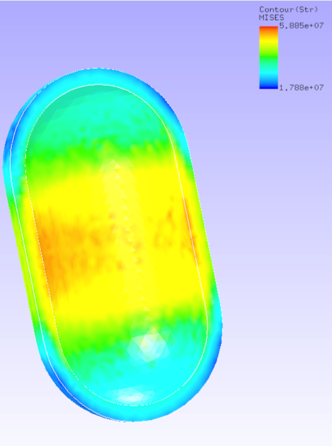
\includegraphics[keepaspectratio,scale=1.5]{images/previous.png}
            \caption{以前の勉強会で報告された結果} \label{fig:previous}
        \end{center}
      \end{figure}
    \end{column}
  \end{columns}
  %
  % TiKZを使った図形の描画 図2でA点を指し示す矢印
  \begin{textblock*}{30pt}(385pt,95pt)
    \begin{tikzpicture}
        \draw[->, draw=cud_red, line width=2pt] (0.7,0.8) -- (0,0.3);
        \node[rectangle,fill=cud_yellow,text width=0.5cm,text centered,rounded corners,minimum height=0.5cm](s) at (1cm,1cm) { \scriptsize A点};
    \end{tikzpicture}
  \end{textblock*}
\end{frame}
